\section{Methodology}
\label{sec:method}
% include the figures path relative to the master file
\graphicspath{ {./content/method/figures/} }
As mentioned in the Sect.\,\ref{sec:descr}, the proposed framework do not rely on pre-processing an segmentation and focus only on feature detection, extraction and classification.
Figure~\ref{fig:framework} illustrates our proposed framework.
    \tikzstyle{block} = [rectangle, draw, fill=blue!40,text = black,
    text width=6em, text centered, rounded corners, minimum height=4em , minimum width = 6em]
    \tikzstyle{myarrow}=[->, thick]
    \tikzstyle{line}=[-, thick]
	\tikzstyle{block2} = [rectangle, draw, fill=white!20,
    text width=6em, text centered, rounded corners, minimum height=4em, minimum width = 6em]
    \tikzstyle{block3} = [rectangle, draw, fill=blue!40, text = black,
    text width=7em, text centered, rounded corners, minimum height=4em , minimum width = 7em]
\def\blockdist{1}
\def\edgedist{1.5}
  %%%% The Framework Sparse Coding 
  \begin{figure}
  
	\begin{tikzpicture}[node distance = 1cm,scale=0.8, every node/.style={scale=0.8}]
%(FEx.east|- FEx.south)
    \node [block2] (input) {Training image};
    \node [block, right of=input,node distance = 2.8cm](PEx){Patch detection};
    \node [block, right of=PEx,node distance = 2.8cm](FEx){Feature extraction};
    	\path (FEx.east)+(+0.8,0) node (g) {};
    	
    	%%% Sparse Coding Block
    \node [block3, right of=g,node distance = 1.7cm](DL){Dictionary learning /KSVD};
    \node [block3, below of=DL,node distance = 2.5cm](PR){Projection};
	%%% 
	\node [block, right of=PR, node distance = 3.6cm](Pool){Pooling};
	\path (Pool.east) + (0.3,0) node (f){}; 
	\path (Pool.east) + (0.2,-0.1) node (f1){};     
    
    \begin{pgfonlayer}{background}
	\path (DL.west |- DL.north)+(-0.4,-0.1+\blockdist) node (a) {};
    \path (PR.east |- PR.south)+(+3.7,-0.7) node (b) {};          
    \path[fill=blue!10,rounded corners, draw=blue!20, dashed] (a) rectangle (b);
\end{pgfonlayer}
	\path (DL.west |- DL.north)+(+2.9,-0.5+\blockdist) node (SP) {\textbf{Sparse Coding}};
	\path (PR.east |- PR.south)+(-1.3,-0.4+\blockdist) node (c){};
	\path (PR.east)+(-3.15,0) node (d) {};
	
	%%% Testing 
	\node [block, below of=FEx, node distance = 2.5cm](FE2){Feature extraction};
	\node [block, below of=PEx, node distance = 2.5cm](PE2){Patch detection};
	\node [block2, below of=input, node distance = 2.5cm](TestImg){Testing image};
	

	
	%%% Classification
	\node [block, right of = Pool, node distance = 3.5cm] (Pre){Prediction}; 
    \node [block, above of = Pre, node distance = 2.5cm] (Learn){Learning}; 
    \begin{pgfonlayer}{background}
	\path (Learn.west |- Learn.north)+(-0.4,-0.1+\blockdist) node (h) {};
    \path (Pre.east |- Pre.south)+(+0.4,-0.7) node (i) {};          
    \path[fill=blue!10,rounded corners, draw=blue!20, dashed] (h) rectangle (i);
\end{pgfonlayer}
	\path (Learn.west |- Learn.north)+(+1.23,-0.5+\blockdist) node (Clas) {\textbf{Classification}};
	\path (Pre.east |- Pre.south)+(-1.3,-0.4+\blockdist) node (j){};
	\path (f1.north)+(0, 2.5) node (k) {};
	\path (Pre.east) + (1.2,0) node (k1) {P(..)}; 
	
    % Draw edges
    \draw [line] (input) -- (PEx) -- (FEx); 
    \draw [myarrow] (FEx)-- (DL);
    \draw [myarrow] (DL) -- (PR) ; 
    \draw [line] (TestImg) -- (PE2) -- (FE2); 
    \draw [myarrow] (FE2) -- (PR) ;
    \draw [line] (PR) -- (Pool); 
    \draw [myarrow] (Pool) -- (Pre); 
    \draw [line] (f1.north) -- + (0,2.5)(k.south); 
    \draw [myarrow] (k.south)+ (0,0.1)  -- (Learn.west); 
    \draw [myarrow] (Pre) -- (k1);

	\end{tikzpicture}

  \caption{The proposed framework.}
  \label{fig:framework}	 	
  \end{figure}

\subsection{Feature extraction}

\subsubsection{Low-level features}
In clinical environment, the prognosis of early stage melanoma relies upon visual cues as stated by the ``ABCDE'' rule.
As introduced in Sect.\,\ref{sec:descr}, this lexicon characterizes cancerous lesions based on their local textures, shapes, and colors from dermoscopic images.
Thus, in order to mimic clinicians assessment, the choice of low-level features encoding similar contextual information is crucial.
In that regard, three low-level features in line with the previous requirements are used and presented into details in the remainder of this section.
Furthermore, these features are locally extracted by partitioning the dermoscopic images into patches.

{\color{red}In clinical environment, the prognosis of early stage melanoma relies upon visual cues, represented by a set of rules such as ``ABCDE''.
One of the main characteristic is variegated colors and difference of color representation between melanoma and benign lesions.
Textural difference, irregular and sharp borders are another valuable and distinguishable tool. 
In this study, three low-level features in line with the previous two discriminative criterion are used.
Color variation criteria is described through two descriptors: opponent color space angle and hue histogram ($C_{1}$) and R,G,B intensities ($C_{2}$).
While the texture, gradient and irregular borders is characterized via \ac{sift} descriptor. 
These descriptors are presented into details in the remainder of this section
Furthermore, these features are locally extracted by partitioning the dermoscopic images into patches.}

% Low-level feature are used to encode the texture and color aspects of dermoscopic images. In this regard, \ac{sift}~\cite{lowe1999object} (named \emph{\ac{sift}}) and two color descriptors: the first color descriptor consists of Hue and opponent color space angle histogram~\cite{van2006coloring}(named \emph{C1}), and the second color descriptor is based on the concatenation of the R, G and B intensities (named \emph{C2}). All these features are extracted from local patches in the dermoscopic images.

\begin{description}
\item[Dense \acf{sift}] descriptors are used to encode the local gradient information using an histogram-based representation~\cite{lowe1999object}. 
\ac{sift} descriptors are extracted over a regular grid such that each grid point is fixed at the center of each image patch.
Typically, a region around the center is divided into $4 \times 4$ sub-regions from which a $8$-bins histogram of the gradient orientations weighted by the gradient magnitudes is computed.
Finally, these histograms are concatenated to build the final descriptor with a final size of $128$ dimensions.
The \ac{sift} implementation used in this work is provided by Vedaldi~\emph{et~al.}~\cite{vedaldi2010vlfeat}.

\item[The opponent color space angle and hue histogram (\emph{C1})] have been first proposed by Van de Weijer and Schmidt as local color features~\cite{van2006coloring}.
These descriptors are robust to photometric variations (i.e., shadow, shading, specularities, and light source changes) as well as geometrical variations (i.e, viewpoint, zoom, and object orientation).
The hue ($H_{\mathcal{O}}$) and angle ($\theta_{\mathcal{O}}$) of opponent color space ($\mathcal{O}_{1,2,3}$) are formulated as shown in Eq.\,\ref{eq:hue} and Eq.\,\ref{eq:theta}, respectively.
The opponent color space transformation is defined as in Eq.\,\ref{eq:opponent}.

\begin{align}
    \begin{pmatrix}
      \mathcal{O}_{1}\\\mathcal{O}_{2} \\\mathcal{O}_{3}
    \end{pmatrix} & =
                    \begin{pmatrix}
                      (R-G)/\sqrt{2}\\
                      (R+G-2B)/\sqrt{6}\\
                      (R+G+B)/\sqrt{3}
                    \end{pmatrix}\ , \label{eq:opponent}\\
    H^{\mathcal{O}} & = \arctan\left(\frac{\sqrt{3}(R-G)}{R+G-2B}\right) \ ,\label{eq:hue}\\
    \theta_{d}^{\mathcal{O}} & = \arctan\left(\frac{\sqrt{3}(R'_{d}-G'_{d})}{R'_{d}+G'_{d}-2B'_{d}}\right)\ , \label{eq:theta}
  \end{align}

\noindent where $d$ denotes the spatial coordinates of ($x$,$y$) and $R'_{d}$, $G'_{d}$, $B'_{d}$ denote the first order derivatives of $RGB$ with respect to the coordinates.

This color descriptor is built by taking a $42$ bins histogram for the opponent angle $\theta^{\mathcal{O}}_{d}$ and the hue channel $H^{\mathcal{O}}$, for a final descriptor size of $84$ dimensions.

\item[The color intensities (\emph{C2})] represent the color information in a simplest form, their intensities.
This descriptor concatenates the color intensities $R$, $G$ and $B$ to create the feature descriptor.
\end{description}

\subsubsection{High-level features}
High-level descriptor is computed using sparse coding techniques. Sparse signal representation has become very popular in the past decades and lead to state-of-the-art results in various applications such as face recognition~\cite{wright2009robust}, image denoising, image inpainting~\cite{elad2006image}, and image classification~\cite{sidibe2015discrimination}. The main goal of sparse modeling is to efficiently represent the images as linear combination of a few typical patterns, called atoms, selected from the dictionary. Here, we intend to use sparse representation of the low-level extracted features for melanoma classification. Sparse coding consists of three main steps: (i) dictionary learning, (ii) low-level features projection, and (iii) feature pooling~\cite{rubinstein2008efficient} (as illustrated in Fig.~\ref{fig:framework}).


\begin{description}
\item[Sparse approximation] Given a dictionary $\mathbf{D} \in \mathbb{R}^{n \times K}$ composed of $K$ atoms and an original signal $\mathbf{y} \in \mathbb{R}^{n}$ (i.e., one feature vector), the sparse approximation corresponds to find the sparest vector $\mathbf{x} \in \mathbb{R}^{K}$ such that:

\begin{equation}
  \argmin_{\mathbf{x}}\|\mathbf{y - Dx} \|_{2} \qquad  \text{s.t.} \  \|\mathbf{x}\|_{0} \leq \lambda \, \label{eq:sprapp}
\end{equation}

\noindent where $\lambda$ is a specified sparsity level.

Solving the above optimization problem is an NP-hard problem~\cite{elad2010sparse}.
However, approximate solutions are obtained using greedy algorithms such as \ac{mp}~\cite{mallat1993matching} or \ac{omp}~\cite{pati1993orthogonal,davis1997adaptive}.
We used the batch-\ac{omp} variant which offers a more efficient algorithm than the standard \ac{omp} for our specific problem~\cite{rubinstein2008efficient}.

\item[Dictionary learning] As stated previously, the sparse approximation is computed given a specific dictionary $\mathbf{D}$, which involves a learning stage from a set of training data.
This dictionary is learned using $K$-\acs*{svd} which is a generalized version of $K$-means clustering and uses \ac{svd}. 
The dictionary is built, by iteratively solving the optimization problem of Eq.\,\ref{eq:dct}, by alternatively computing the sparse approximation of $\mathbf{X}$ and the dictionary $\mathbf{D}$.

\begin{equation}
  \argmin_{\mathbf{D,X}} \|\mathbf{Y} - \mathbf{D}\mathbf{X}\|_{2} \qquad  \text{s.t.} \  \|\mathbf{x}_{i}\|_{1} \leq \lambda \,\label{eq:dct}
\end{equation}

\noindent where $\mathbf{Y}$ is a training set of low-level descriptors, $\mathbf{X}$ is the associated sparse coded matrix (i.e., set of high-level descriptors) with a sparsity level $\lambda$, and $\mathbf{D}$ is the dictionary with $K$ atoms.

Given $\mathbf{D}$, $\mathbf{X}$ is computed using the batch-\ac{omp} algorithm, while given $\mathbf{X}$, $\mathbf{D}$ is sequentially updated, one atom at a time using \ac{svd}. 

\item[Low-level features projection] Once the dictionary is learned, each set of low-level features $\mathbf{F}_{I} \in \mathbb{R}^{n \times p}$ extracted from $p$ patches in an image is encoded using the dictionary $\mathbf{D}$, solving the optimization problem presented in Eq.\,\ref{eq:sprapp} such that $\mathbf{F}_{I} \simeq \mathbf{DX}_{I}$.

\item[Feature pooling] The sparse coded matrix $\mathbf{X}_{I}$ is max-pooled to build a final descriptor $\mathbf{f}$ characterizing the given image, such that:

\begin{equation}
  \mathbf{f}_i = \max_{j}\left(|\mathbf{X}_{I}(i,j)|\right), \ \forall i = 1, \cdots, K\ .
\end{equation}

% This set is further max-pooled to built a final global descriptor to characterize the whole image.

\end{description}
Figure~\ref{fig:sparsecoding} illustrate the training and testing stage, using sparse coded features.
\begin{figure}
\begin{center}
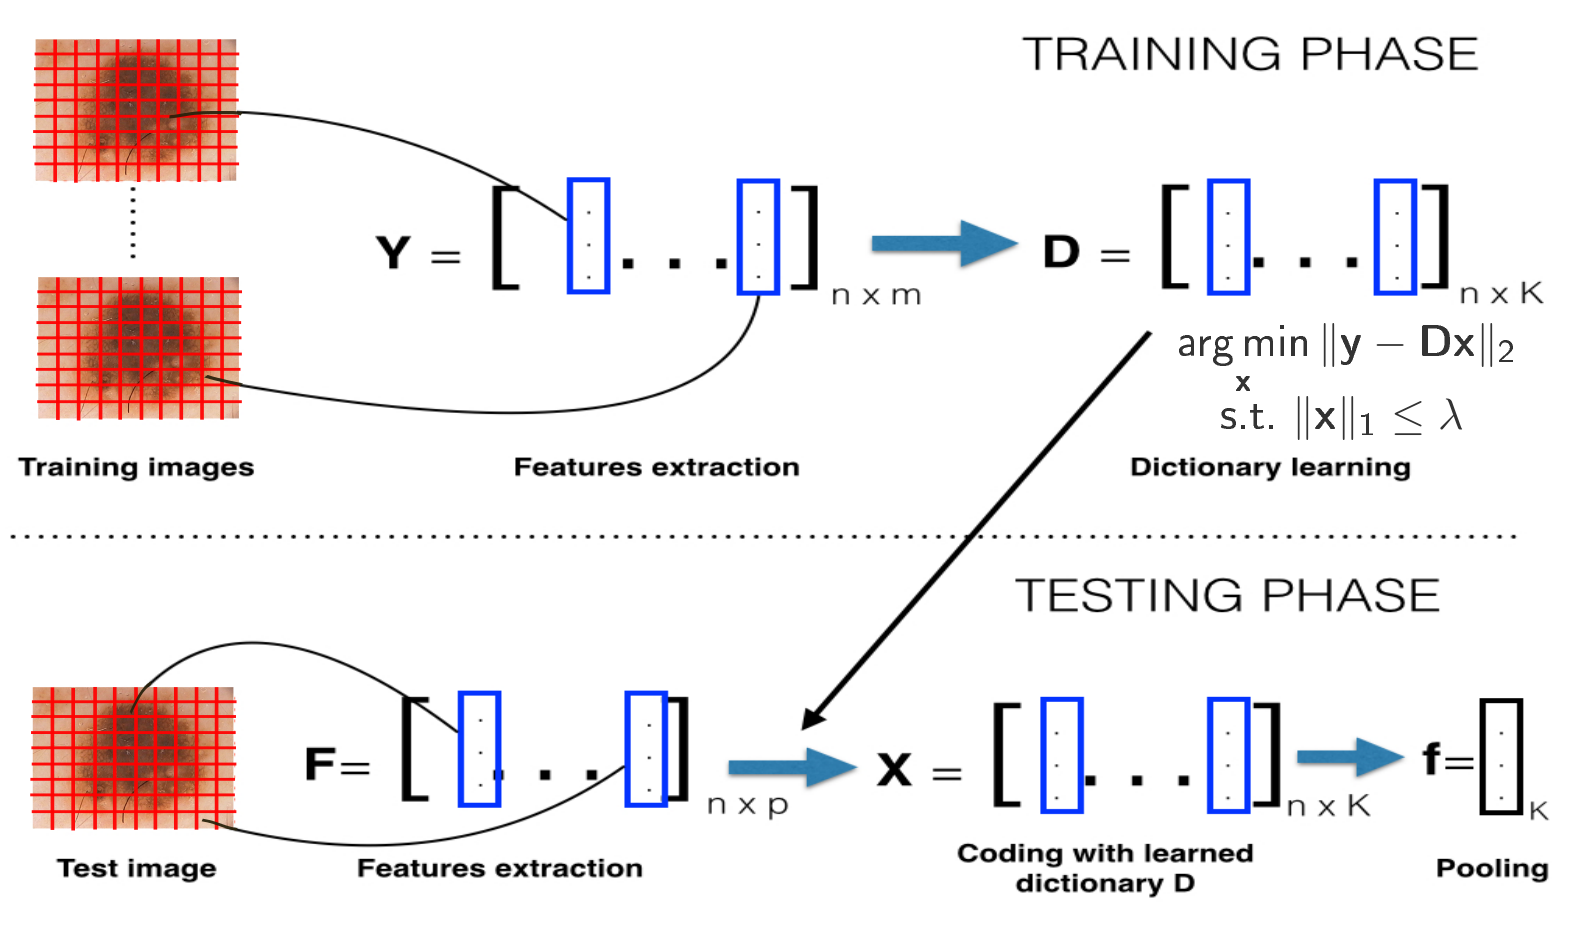
\includegraphics[width = 0.8\textwidth]{sparse-coding-melanoma.png}
\end{center}
\caption{Sparse coded representation for training and testing samples.}
\label{fig:sparsecoding}
\end{figure}
\subsection{Feature classification}

\subsubsection{Over-sampling from imbalanced dataset}

Similarly to Barata~\emph{et~al.}\cite{barata2013two}, the imbalanced issue of the dataset is tackled by over-sampling the samples of the minority class.
New samples are generated to get a balanced set by randomly repeating original samples of the minority class with an additional Gaussian noise $\mathcal{N}(0, 0.0001)$.

\subsubsection{\acf*{rf}}

The classification is performed using a \ac{rf} classifier.
\Ac{rf} is an ensemble of decision trees~\cite{breiman2001random} which generalizes the classification process by applying two types of randomization: at the tree level, each tree is fed by a bootstrap made of $S'$ samples built from the original data of size $S$ such that  $S=S'$, and at the node level, a subset of feature dimensions $m$ is randomly selected from the original dimension $M$ such that $m=\sqrt{M}$. 
The trees in \ac{rf} are grown to their maximum length without any pruning.
Each tree in the ensemble casts a unit vote in the final prediction and the final prediction is based on combination of all the votes. 
\Ac{rf} is used with 1000 un-pruned trees using gini criterion and the original feature dimension.

% \section{Contribution}
% We propose a classification framework which do not rely on pre-processing and lesion segmentation and is based on sparse coded features. It is also presented that low-level features such as intensity values can be used directly for classification of the lesions within such framework. 




%%% Local Variables: 
%%% mode: latex
%%% TeX-master: "../../master"
%%% End: 
